% Build:  cd paper && latexmk -pdf main.tex   (or upload this folder to Overleaf)
% Before submitting, this must find only the \newcommand line:  grep -n "todo" main.tex
\documentclass[10pt,a4paper,twocolumn]{article}
\usepackage[margin=2cm,columnsep=0.6cm]{geometry}
\usepackage[T1]{fontenc}
\usepackage[utf8]{inputenc}
\usepackage{times}
\usepackage{amsmath}
\usepackage{booktabs}
\usepackage{graphicx}
\usepackage{xcolor}
\usepackage[numbers,sort&compress]{natbib}
\usepackage{url}
\usepackage[colorlinks=true,allcolors=blue!60!black]{hyperref}

\newcommand{\todo}[1]{\textcolor{red}{\textbf{[TODO: #1]}}}
\newcommand{\model}[1]{\texttt{#1}}

\title{When Retrieval Misses a Hop: Retrieval Quality, Hallucination, and Training-Free Abstention in Multi-Hop RAG}
\author{Bobburi Divakara\\
Department of Artificial Intelligence and Data Science\\
CMR Institute of Technology, Bengaluru, India\\
\todo{contact email}}
\date{}

\begin{document}
\maketitle

\begin{abstract}
Retrieval-augmented generation (RAG) is meant to ground a model's answers in evidence, but it does
not guarantee that the answers stay faithful to the retrieved passages. We measure how retrieval
quality affects hallucination for two small open-weight models on 100 multi-hop HotpotQA questions,
under six conditions from no retrieval to perfect retrieval (1,200 answers), and we test whether a
rule that needs no model training can reduce hallucination by withholding answers. Hallucination
depends strongly on whether retrieval found every hop. With both gold passages in the top five, 7.0\%
and 4.5\% of the answers of the two models are hallucinated. With only one, the rates are 63.1\% and
77.7\%, and the gap persists when the same question is compared with itself. Differences between
retrievers are smaller and their intervals overlap. Retrieval confidence does not work as an abstention
signal: the score of the top passage is near chance (AUROC 0.46--0.54). A simple check of whether the
answer's words appear in the passages does better (AUROC 0.75--0.77 for one model, 0.60--0.63 for the
other). In the best case it lowers hallucination from 21.3\% to 11.0\% at 74.9\% coverage, at a cost in
correct answers, and it helps much less when a model picks wrong spans from the context. A human check of 100 answers
agrees only moderately with the LLM judge ($\kappa=0.54$) and suggests that absolute rates may be too high, but it
preserves the gap between one and two gold passages.
\end{abstract}

\section{Introduction}

Language models can state false information with confidence \cite{ji2023survey}. RAG addresses this by
giving the model passages from a document collection and asking it to answer from them
\cite{lewis2020rag}. This does not remove the problem: when the retriever returns the wrong passages, the
generator builds on bad evidence \cite{yan2024crag}, and answers can include claims that the passages do
not back \cite{niu2024ragtruth}.

Multi-hop questions make this failure easy to see, because retrieval can succeed partly. A question that
needs two passages can get one of them, and the model then has some relevant context but not enough to
answer. Common ranking metrics can hide this: a system can place one relevant passage near the top for
most questions and still often miss the second.

Self-RAG \cite{asai2024selfrag} and CRAG \cite{yan2024crag} decide when to trust retrieval, but both depend
on a fine-tuned component. That rules them out when a model is only reachable through an API, or when there
is no budget for training. We therefore ask two questions:
\begin{description}
\item[RQ1:] How does retrieval quality affect hallucination (faithfulness) in RAG with small open-weight
  models?
\item[RQ2:] Can a training-free rule that abstains when a confidence signal is low reduce hallucination
  without losing many correct answers?
\end{description}

Our contributions are: (1) a measurement of hallucination across six retrieval conditions for two models,
with intervals and a same-question comparison; (2) evidence that the number of gold passages found is far
more informative than the choice of retriever; (3) a negative result for retrieval scores as an abstention
signal, and a partial positive result for a simple lexical check, with its cost reported on held-out data.
The code, generated answers, judge verdicts and result tables are public.\footnote{\url{https://github.com/Diwakar-Bobburi/rag-hallucination-study}}

\section{Related Work}

\textbf{Measuring faithfulness.} RAGAS \cite{es2024ragas} evaluates RAG without reference answers, using an
LLM to check an answer's statements against the context. RAGTruth \cite{niu2024ragtruth} provides human
hallucination labels for RAG outputs and separates conflicts with the context from baseless information. We
adapt the first method and the label scheme of the second.

\textbf{Reducing hallucination.} Self-RAG \cite{asai2024selfrag} trains a model to emit reflection tokens that
control retrieval and critique its output. CRAG \cite{yan2024crag} trains an evaluator that scores retrieved
documents and triggers refinement or web search. Both show the value of deciding when to trust retrieval, and
both need fine-tuning. Abstaining is a form of selective prediction, which trades coverage against quality
\cite{geifman2017selective}.

\textbf{Detecting unsupported answers.} Recent work is close to ours in aim. HALT-RAG
\cite{goswami2025halt} combines NLI models and lexical signals in a trained, calibrated meta-classifier that
supports abstention. \citet{bouke2026context} proposes a training-free detector that compares a sentence's
likelihood with and without each source chunk, and finds it weakest on short-answer QA, where the scorer can
answer from memory. \citet{sinha2025semantic} reports that embedding-based detectors fail on real hallucinations
from aligned models. Our study differs in scope rather than in sophistication: we compare very cheap signals
that any pipeline already has, and we tie their usefulness to the error profile of each generator on multi-hop
questions. We do not claim that such signals have never been studied.
\todo{Run and document a fuller literature search before submitting. The papers above came from one search.}

\section{Method}

\subsection{Data}
We use the distractor configuration of HotpotQA \cite{yang2018hotpotqa}, validation split, in which all questions
have the level ``hard''. We sample 500 questions (seed 42; 404 bridge, 96 comparison) and evaluate retrieval on all
of them. Because of API limits, generation and judging use the first 100 (79 bridge, 21 comparison). The corpus
holds the paragraphs of the 500 questions and of 1,500 further questions that are never asked, giving 19,225
passages of about 92 words each. Every question has two gold passages.

\subsection{Retrievers and Conditions}
We compare four retrievers and pass the top $k=5$ passages to the generator, in retrieval order. \emph{BM25}
\cite{robertson2009bm25} is keyword search. \emph{Dense} \cite{karpukhin2020dpr} uses \model{BAAI/bge-small-en-v1.5}
\cite{xiao2024cpack} with a FAISS inner-product index \cite{johnson2021faiss}. \emph{Hybrid} fuses the top 100 passages of
both with reciprocal rank fusion \cite{cormack2009rrf} ($k=60$). \emph{Hybrid+rerank} re-scores the top 20 hybrid passages
with the cross-encoder \model{cross-encoder/ms-marco-MiniLM-L-6-v2} \cite{reimers2019sbert,nogueira2019rerank}. Two
further conditions mark the limits: \emph{closed-book} (no passages) and \emph{oracle} (only the two gold passages).

\subsection{Generators}
The generators are \model{openai/gpt-oss-20b} \cite{openai2025gptoss} (reasoning effort low) and
\model{qwen/qwen3.8-27b} \cite{qwen2026qwen38} (reasoning effort none), both through the Groq API with temperature 0 and at
most 2,048 tokens. The 100 questions, six conditions and two models give 1,200 answers. The prompt asks for a short answer
using only the context. It does not offer ``I don't know'' as an option, so any refusal is the model's own. Refusals are
detected with a list of phrases and count as abstained.

\subsection{Metrics}
\textbf{Retrieval.} Recall@$k$ is the share of gold passages in the top $k$. Both@$k$ is the share of questions with both
gold passages in the top $k$. MRR uses the rank of the first gold passage.

\textbf{Accuracy.} Exact match (EM) and F1 follow the HotpotQA script \cite{yang2018hotpotqa}. An answer counts as \emph{correct}
if $\text{F1}\geq0.5$ and the model did not abstain.

\textbf{Faithfulness.} A judge labels each answer as \emph{supported} (the context states or clearly implies it),
\emph{contradicted} (the context conflicts with it) or \emph{unsupported} (the context does not contain enough to back it), after
RAGTruth \cite{niu2024ragtruth}. The judge is adapted from RAGAS \cite{es2024ragas}, judges the whole short answer in one call, and is
told to use only the context. The \emph{hallucination rate} is the share of non-abstained answers labelled contradicted or
unsupported. This measures faithfulness to the passages, not truth: a hallucinated answer can be correct.
No answer is marked supported merely because its text appears in the passages. Closed-book answers are not judged.

The main judge is \model{gemma-4-31b-it} \cite{gemma2026gemma4}, from a different model family than both generators. All tables use
this judge. A second judge, \model{openai/gpt-oss-120b} \cite{openai2025gptoss}, is used only to measure agreement. Of 968 non-abstained
answers with context, 19 (2.0\%) got no readable verdict from the main judge and are excluded.
Agreement is reported as percentage and as Cohen's $\kappa$ \cite{cohen1960kappa}.
To check the judges, we drew a balanced sample of 100 answers in random order, 50 that the main judge called hallucinated and 50 it called supported, so agreement on it is not agreement at the natural rate of hallucination. The author labelled all of them, from the passages only, in a tool that hid the judges' labels. The author was not fully naive: before labelling, the author knew the pooled results and the sampling scheme, and had been told that a model reader found the judge stricter than itself, and the last 20 answers were labelled after the results of the first 80 were known. As a further check, a third model, Claude Opus 5.5, labelled all 100 under the same blinding. It is not independent of the study either: it helped to draft this paper, and it had seen the pooled results, the sampling scheme and one judge reason.

\textbf{Uncertainty.} Intervals are 95\% percentile bootstrap intervals \cite{efron1993bootstrap} with 2,000 resamples of answers.
Within one condition each answer is a different question. Pooled tables repeat questions, so we also report intervals that resample
whole questions.

\subsection{Abstention Rule}
The rule withholds an answer when a signal is below a threshold $\tau$. It needs no model training and no change to the generator, and
is applied to the saved answers. We test three signals. \emph{top1} and \emph{top2} are the retriever or reranker scores of the best
and second-best passage; a weak second passage might indicate a missing hop. \emph{answer\_overlap} is the share of the answer's
normalised words that appear in the passages shown. ``Yes'' and ``no'' answers get 1.0 and are never withheld, since those words say
nothing about support.

We choose $\tau$ on a random 50\% development split to maximise $(\#\text{correct}-\#\text{hallucinated})/n$, with ties going to
higher coverage, and evaluate on the other half. A split this small is noisy, so we report the mean over 200 random splits. The
standard deviation describes variation between overlapping splits and is not a confidence interval. AUROC is computed on all answers,
with hallucinated answers as the negative class, so 0.5 is chance. Coverage counts answers kept out of all questions. Accuracy after
abstention counts a withheld answer as wrong. The rule is training-free but not label-free: choosing $\tau$ needs about 50 labelled answers.

\section{Results}

\begin{table}[t]
\centering\small
\caption{Retrieval quality on all 500 questions, plus Both@5 on the 100 questions used for generation.}\label{tab:retrieval}
\begin{tabular}{@{}lrrrrr@{}}
\toprule
 & \multicolumn{4}{c}{All 500} & First 100 \\
\cmidrule(lr){2-5}
Retriever & R@5 & Both@5 & Both@10 & MRR & Both@5 \\
\midrule
BM25 & 0.696 & 0.428 & 0.600 & 0.865 & 0.47 \\
Dense & 0.826 & 0.666 & 0.764 & 0.918 & 0.64 \\
Hybrid & 0.812 & 0.630 & 0.766 & 0.916 & 0.67 \\
Hybrid+rerank & 0.834 & 0.670 & 0.814 & 0.948 & 0.71 \\
\bottomrule
\end{tabular}
\end{table}

\begin{table*}[t]
\centering\footnotesize
\caption{Answer quality and hallucination by condition (100 questions per cell; judge \model{gemma-4-31b-it}). Abst.: answers the model
itself declined (\%). $n$: judged answers. Hall.: hallucination rate (\%) with 95\% bootstrap interval. Contr.: share labelled
contradicted (\%); the rest of Hall.\ is unsupported.}\label{tab:main}
\begin{tabular}{@{}lrrrrlrcrrrrlr@{}}
\toprule
 & \multicolumn{6}{c}{\model{gpt-oss-20b}} & & \multicolumn{6}{c}{\model{qwen3.8-27b}} \\
\cmidrule{2-7}\cmidrule{9-14}
Condition & EM & F1 & Abst. & $n$ & Hall.\ [CI] & Contr. & & EM & F1 & Abst. & $n$ & Hall.\ [CI] & Contr. \\
\midrule
Closed-book & 0.19 & 0.29 & 0 & -- & -- & -- & & 0.21 & 0.28 & 0 & -- & -- & -- \\
BM25 & 0.42 & 0.57 & 11 & 88 & 34.1 [25.0, 43.2] & 1.1 & & 0.54 & 0.66 & 1 & 97 & 42.3 [32.0, 51.6] & 3.1 \\
Dense & 0.52 & 0.66 & 8 & 90 & 21.1 [13.3, 30.0] & 1.1 & & 0.66 & 0.76 & 1 & 96 & 28.1 [19.8, 37.5] & 1.0 \\
Hybrid & 0.51 & 0.67 & 4 & 93 & 23.7 [15.1, 32.3] & 1.1 & & 0.61 & 0.73 & 1 & 97 & 29.9 [21.6, 39.2] & 4.1 \\
Hybrid+rerank & 0.51 & 0.67 & 2 & 96 & 25.0 [16.7, 34.4] & 2.1 & & 0.63 & 0.74 & 2 & 96 & 25.0 [16.7, 34.4] & 2.1 \\
Oracle & 0.65 & 0.79 & 1 & 98 & 8.2 [3.1, 13.3] & 3.1 & & 0.73 & 0.84 & 1 & 98 & 6.1 [2.0, 11.2] & 1.0 \\
\bottomrule
\end{tabular}
\end{table*}

\subsection{Retrieval Quality}
Table~\ref{tab:retrieval} shows that finding one relevant passage is much easier than finding both. MRR is high for every retriever
(0.865--0.948), yet Both@5 is only 0.428 for BM25 and 0.670 for hybrid+rerank. Even the best retriever misses a hop for about a third
of the questions. The 100 questions used for generation are not a perfect sample of the 500: dense and hybrid swap order on them, so we
draw no ranking of those two.

\subsection{Hallucination by Condition}
Table~\ref{tab:main} gives the main results. Retrieval helps accuracy: EM rises from 0.19 and 0.21 closed-book to at best 0.52 and 0.66 with
a retriever, and 0.65 and 0.73 with the oracle. Hallucination is highest for BM25 (34.1\% and 42.3\%) and lowest for the oracle (8.2\% and
6.1\%). The intervals of the four retrievers overlap for both models, including BM25 against dense, so we do not rank them. Nor does better
Both@5 translate neatly at this scale: hybrid+rerank has the highest Both@5 on these questions, but for \model{gpt-oss-20b} its rate is not
below dense.

Almost all hallucinations are unsupported, not contradicted. Of 949 judged answers, 230 are hallucinated: 211 unsupported and 19 contradicted.
The models rarely state something the passages conflict with; they more often state something the passages do not establish.

\subsection{Effect of Gold Passages Found}

\begin{table}[t]
\centering\small
\caption{Hallucination by the number of gold passages in the top 5 (four retrievers pooled). $n$: judged answers. Intervals resample answers,
and so are too narrow for the pooled rows; see the text for intervals that resample questions.}\label{tab:gold}
\begin{tabular}{@{}llrlr@{}}
\toprule
Model & Gold & $n$ & Hall.\ \% [CI] & EM \\
\midrule
\model{gpt-oss} & 0 of 2 & 1 & -- & -- \\
 & 1 of 2 & 122 & 63.1 [54.9, 71.3] & 0.30 \\
 & 2 of 2 & 244 & 7.0 [3.7, 10.2] & 0.63 \\
 & Oracle & 98 & 8.2 [3.1, 13.3] & 0.65 \\
\midrule
\model{qwen} & 0 of 2 & 2 & -- & -- \\
 & 1 of 2 & 139 & 77.7 [70.5, 84.2] & 0.37 \\
 & 2 of 2 & 245 & 4.5 [2.0, 7.3] & 0.76 \\
 & Oracle & 98 & 6.1 [2.0, 11.2] & 0.73 \\
\bottomrule
\end{tabular}
\end{table}

\begin{figure}[t]
\centering
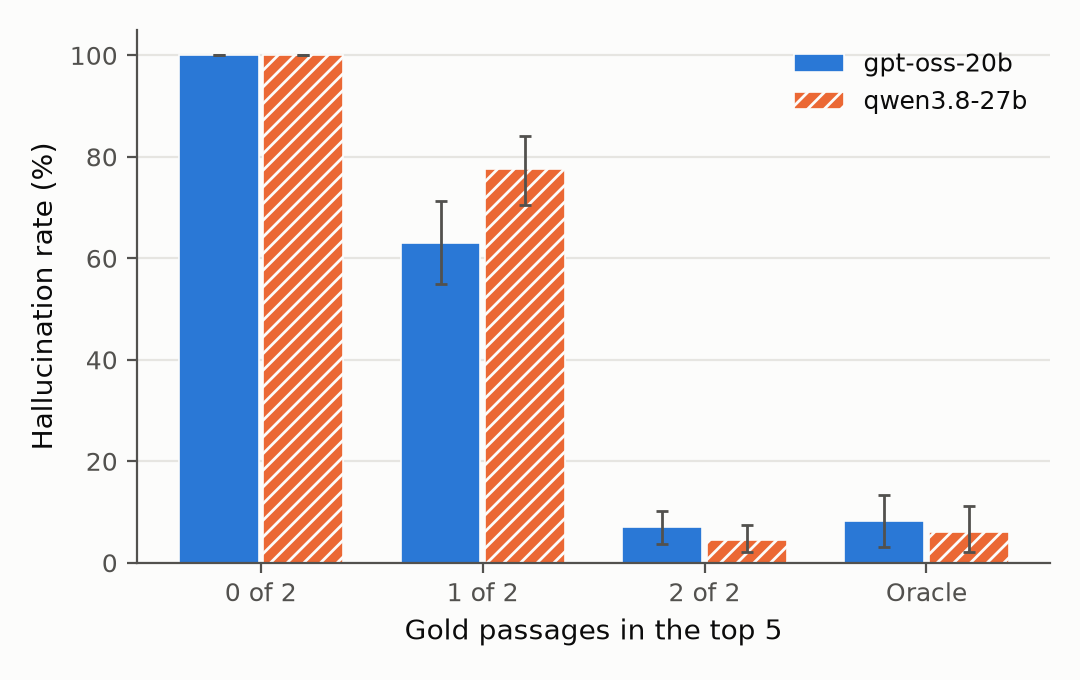
\includegraphics[width=\columnwidth]{fig_gold_found.png}
\caption{Hallucination by gold passages in the top 5. The ``0 of 2'' bars rest on 1 and 2 answers and should not be interpreted. Error bars
resample answers.}\label{fig:gold}
\end{figure}

Table~\ref{tab:gold} and Figure~\ref{fig:gold} hold the key result for RQ1. With both gold passages in the top five, 7.0\% and 4.5\% of answers
are hallucinated, in line with the oracle. With only one, the rates are 63.1\% and 77.7\%. Retrieval found neither passage in only 3 cases, too
few to interpret.

Because the table pools four retrievers, one question can appear up to four times. Resampling whole questions widens the intervals but does not
close the gap: for one gold passage, [48.4, 77.0] and [65.7, 88.3]; for two, [2.7, 12.0] and [0.8, 9.3]. Two further checks address whether questions
with a missed hop are simply harder. First, some questions are harder: under the oracle, questions with a one-gold retrieval reach 15.7\% and 8.5\%
hallucination, against 5.1\% and 3.8\% for questions with a two-gold retrieval. That difference is far smaller than the one in Table~\ref{tab:gold}.
Second, on questions where retrievers disagree, each question can be compared with itself. On those 32 and 40 questions, hallucination is 64.1\% and 78.3\%
with one gold passage and 10.4\% and 5.0\% with two. This remains observational, but difficulty alone does not explain the effect.

The result is partly built into the definition: with a hop missing, the passages can rarely support the answer. What the data add is the models'
behaviour in that state. The prompt offered no explicit way to decline, but it did tell the models to use only the context, and they rarely refused.
Self-abstention never exceeds 11\% in any condition and is 1--2\% for \model{qwen3.8-27b} when it is given passages. A missing hop usually leads to an answer anyway.

\subsection{Abstention (RQ2)}

\begin{table*}[t]
\centering\small
\caption{Abstention on held-out data, as the mean over 200 random dev/test splits (each test half has about 49 questions). Coverage, Hall.\ and Acc.\ in \%; SD over
splits in brackets. Removed: hallucinations withheld per test half. Lost: correct answers withheld per test half. ``Before'' values are averaged over test halves, so they
differ slightly from Table~\ref{tab:main}.}\label{tab:abstention}
\begin{tabular}{@{}lllrrrlrrrr@{}}
\toprule
Retriever & Model & Signal & AUROC & Coverage & Hall.\ before & Hall.\ after (SD) & Removed & Lost & Acc.\ before & Acc.\ after \\
\midrule
Hybrid+rerank & \model{gpt-oss} & top1 & 0.50 & 95.9 & 25.4 & 25.9 (4.1) & 0.0 & 0.4 & 71.4 & 70.6 \\
 & & top2 & 0.57 & 93.9 & 25.4 & 24.3 (4.5) & 1.0 & 1.5 & 71.4 & 68.3 \\
 & & answer\_overlap & 0.75 & 81.8 & 25.4 & 17.1 (4.9) & 5.3 & 3.2 & 71.4 & 65.0 \\
 & \model{qwen} & top1 & 0.48 & 96.3 & 25.2 & 25.2 (4.5) & 0.2 & 0.2 & 77.3 & 76.9 \\
 & & top2 & 0.54 & 93.8 & 25.2 & 25.0 (4.4) & 0.6 & 1.4 & 77.3 & 74.4 \\
 & & answer\_overlap & 0.60 & 91.5 & 25.2 & 22.3 (5.0) & 2.0 & 1.5 & 77.3 & 74.3 \\
\midrule
Dense & \model{gpt-oss} & top1 & 0.54 & 89.1 & 21.3 & 21.4 (4.5) & 0.2 & 1.1 & 69.6 & 67.5 \\
 & & top2 & 0.68 & 86.0 & 21.3 & 19.2 (5.3) & 1.4 & 1.7 & 69.6 & 66.2 \\
 & & answer\_overlap & 0.77 & 74.9 & 21.3 & 11.0 (4.9) & 5.5 & 2.8 & 69.6 & 63.9 \\
 & \model{qwen} & top1 & 0.46 & 98.0 & 28.2 & 28.4 (4.7) & 0.0 & 0.5 & 79.0 & 78.1 \\
 & & top2 & 0.53 & 96.2 & 28.2 & 27.7 (4.9) & 0.6 & 1.1 & 79.0 & 76.7 \\
 & & answer\_overlap & 0.63 & 90.2 & 28.2 & 23.2 (5.5) & 3.4 & 2.3 & 79.0 & 74.3 \\
\bottomrule
\end{tabular}
\end{table*}

\begin{figure}[t]
\centering
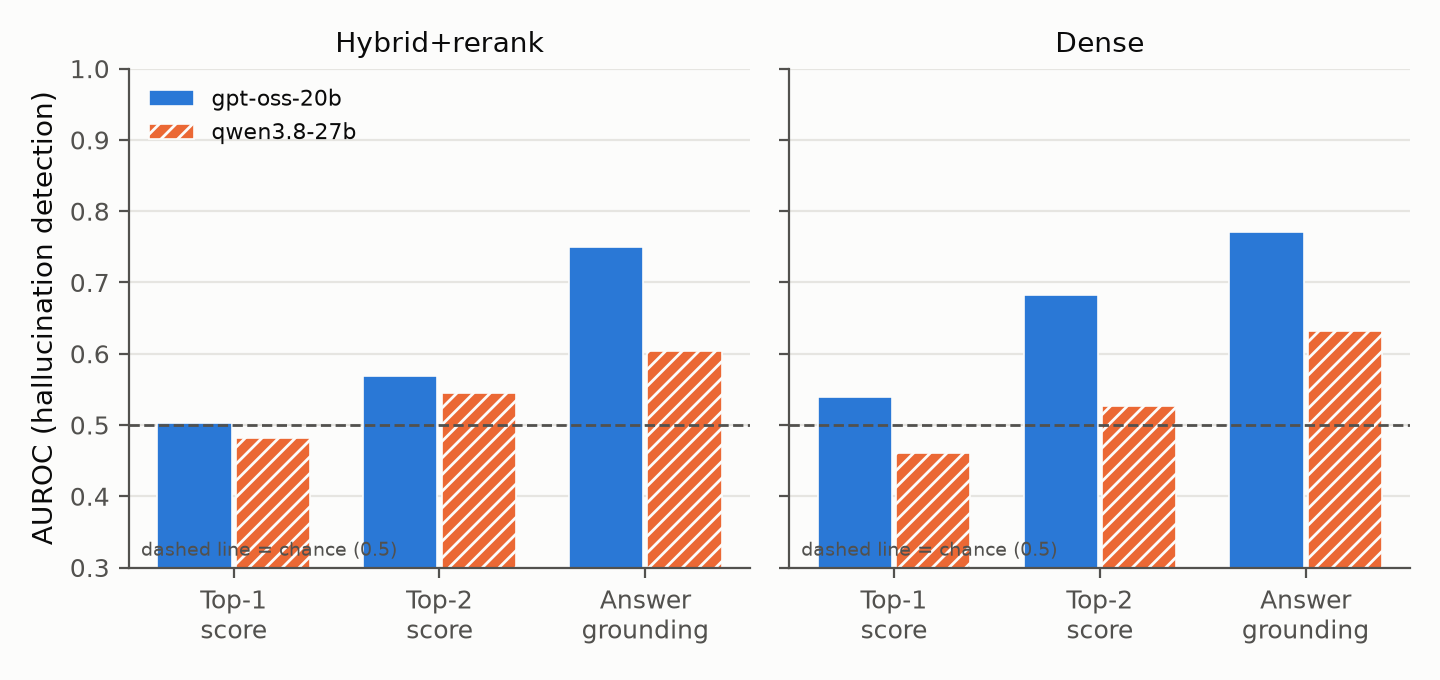
\includegraphics[width=\columnwidth]{fig_abstention.png}
\caption{AUROC of each signal. The vertical axis starts at 0.3; the dashed line marks chance.}\label{fig:abstention}
\end{figure}

\textbf{Retrieval confidence does not work.} The top1 score is near chance everywhere (AUROC 0.46--0.54), and removes almost no hallucinations
(Table~\ref{tab:abstention}, Figure~\ref{fig:abstention}). The top2 score is better in one case (0.68, \model{gpt-oss-20b} with dense) but ranges from 0.53 to
0.68, and the thresholds chosen for it keep most answers and change hallucination by little. A likely reason, which we did not test directly, is that the
score reflects how well a passage matches the question, and a strong match to one hop says little about whether the other was found.

\textbf{The grounding check helps, unevenly.} The answer\_overlap signal reaches AUROC 0.75--0.77 for \model{gpt-oss-20b} and 0.60--0.63 for \model{qwen3.8-27b}. Its
best case is \model{gpt-oss-20b} with dense, where hallucination falls from 21.3\% to 11.0\% at 74.9\% coverage. The cost is real: per test half it withholds 5.5
hallucinations and 2.8 correct answers, and accuracy falls from 69.6\% to 63.9\%. For \model{qwen3.8-27b} the gain is much smaller (28.2\% to 23.2\% with dense).

\section{Analysis}

\subsection{Where Hallucinated Answers Come From}
The difference between the two models follows from their errors. For \model{qwen3.8-27b}, all words of the answer appear in the context in 91 of 127
hallucinated answers (72\%), against 48 of 103 (47\%) for \model{gpt-oss-20b}. This suggests that Qwen more often answers with a span from the passages that they do not back, which a lexical check cannot see. It would also
explain why the grounding check works better for the model whose hallucinations more often contain words from outside the context.

Faithfulness and correctness also come apart. Of the 230 hallucinated answers, 124 (54\%) are nevertheless correct by the F1 threshold (57 of 103 and 67 of 127).
This fits the models filling a missing hop from what they already know, or guessing well, although we cannot separate the two from these counts.
Conversely, 110 of 719 supported answers (15\%) are incorrect. A check for faithfulness cannot replace a check for accuracy, nor the reverse.

Pooled across conditions, comparison questions hallucinate less than bridge questions (11.7\% against 25.1\% and 9.7\% against 30.7\%), but this does not hold for BM25,
where comparison questions reach 40.0\% and 38.1\%. There are only 21 comparison questions per condition, so we treat this as suggestive.

To look at causes directly, the author and Claude Opus 5.5 each assigned 30 hallucinated answers from the BM25 and dense conditions to one cause, both seeing the judge's label and reason and the gold answer, so this step is not blind. Causes overlap. The author chose among the five names in the labelling tool, and the model followed one rule in order: the answer is actually backed (judge error); the needed facts are present but the answer does not follow (passage misread); a needed fact is absent and the answer's words are not in the passages (answer from memory); a needed fact is absent and the answer comes from the passages, is yes/no, or is ``None'' (one hop missing); no relevant passage at all (wrong passage retrieved). The author's counts are 18 one hop missing, 8 wrong passage retrieved, 3 passage misread, 1 judge error and 0 answer from memory; the model's are 18 one hop missing, 7 answer from memory, 4 judge error, 1 passage misread and 0 wrong passage retrieved. They give the same cause for only 12 of 30 answers ($\kappa=0.05$), so individual causes are not reliable. A coarser reading is shared, although we made this grouping after seeing the results: the author attributes 26 answers to evidence missing from the context (one hop missing or wrong passage retrieved), the model 25 (one hop missing or answer from memory), and they overlap on 24. Of the 30 answers, 27 had one gold passage in the top five, including all 26 of the author's, which fits the view that a missing hop is the main route to hallucination. The author's single judge error does not fit the human check, where 20 of 50 answers the judge called hallucinated were labelled supported. Six answers are on both sheets: the author labelled 3 supported and gave only 1 of those the cause judge error. The cause step showed the judge's reason, which may have influenced the author.

\subsection{Judge Reliability}
The two LLM judges agree on 92.3\% of 663 shared answers with binary labels ($\kappa=0.81$) and 90.5\% with three labels ($\kappa=0.77$). Agreement between models does not show that
either is right, and the second judge shares a family with one generator.


\textbf{Human check.} The author agrees with the main judge on 77.0\% of 100 answers with binary labels ($\kappa=0.54$) and 73.0\% with three labels ($\kappa=0.48$), and with the second judge on 78.5\% of the 79 answers it covered ($\kappa=0.54$) and 77.2\% with three labels ($\kappa=0.52$). This is moderate agreement, clearly lower than between the two judges, although the balanced sample means the values are not directly comparable. The disagreements are one-sided: of 23 binary disagreements with the main judge, the judge called 20 hallucinated where the author called them supported, and only 3 the other way round. Reweighting the sample to the observed rate gives about 19.1\% hallucination overall against the judge's 24.2\%.

There are two readings of this gap, and we cannot separate them. The judge may be too strict: it sometimes faults an answer for wording in the question. The author may also be too lenient: in 10 of those 20 cases, both judges and the third-model reader all called the answer hallucinated. We therefore treat the absolute rates in Table~\ref{tab:main} as uncertain and possibly too high.

The main result does not depend on this. Using the author's labels, 26 of 42 answers with one gold passage are hallucinated, against 3 of 42 with both (about 54\% and 4\% after reweighting within each group). These are small, balanced subsets, so they support the direction and size of the gap rather than exact values.

\textbf{Third-model reader.} Claude Opus 5.5 agrees with the main judge on 86.0\% of 100 answers with binary labels ($\kappa=0.72$) and 82.0\% with three labels ($\kappa=0.67$), and with the second judge on 82.3\% of 79 answers ($\kappa=0.64$) and 77.2\% with three labels ($\kappa=0.56$). It agrees with the author on 77.0\% of 100 answers ($\kappa=0.51$). Models agree more with each other than with the human rater, so agreement between models should not be taken as evidence of accuracy.

\section{Discussion}

\textbf{RQ1.} Whether retrieval found every hop matters much more than which retriever was used. This points to a practical shift in evaluation: for multi-hop questions, track Both@$k$ alongside
MRR, since MRR was high here even where a hop was often missing. It also suggests that improving second-hop recall, for example with iterative retrieval, is a promising target, though we did not test that here.

\textbf{RQ2.} A training-free rule can reduce hallucination, but not with the signal that pipelines most readily have. Retrieval scores should not be assumed to indicate whether an answer is supported.
The grounding check needs only string operations after generation, but its benefit depends on the model and it can catch only answers with words from outside the context. It costs correct answers, partly because
54\% of hallucinated answers are correct by F1: withholding them improves faithfulness at the expense of accuracy. Whether that trade is worthwhile depends on the application. We compare with Self-RAG and CRAG only in requirements, as we did not run them on this data.

\section{Limitations}
\begin{itemize}\setlength\itemsep{1pt}
\item \textbf{Small sample.} There are 100 questions per condition, intervals are wide, and retriever differences overlap. We did not run paired significance tests between retrievers. Abstention rests on test halves of about 49 questions.
\item \textbf{Observational.} The number of gold passages found was not assigned at random. Our same-question check reduces the concern about difficulty, but it covers only questions where retrievers disagree, and those may differ from the rest.
\item \textbf{An LLM as judge.} Labels come from a model that can make mistakes, and every hallucination rate depends on them. Agreement with the human check was only moderate ($\kappa=0.54$), that check covers 100 answers by one rater who knew the study's results, and it suggests the absolute rates may be too high. Answers with unreadable verdicts are few (2.0\%), but they may not be missing at random.
\item \textbf{Faithfulness is not truth.} A supported answer may be wrong, and an unsupported one may be true.
\item \textbf{Different context sizes.} The oracle shows two passages and retrievers show five, and passage order can affect models \cite{liu2024lost}.
\item \textbf{Abstained answers are excluded} from the hallucination rate, and the rates of abstention differ between conditions (up to 11\%), which can slightly affect comparisons.
\item \textbf{Generality.} This is one Wikipedia-based data set with short answers, and two models. The lexical check suits short answers, and it may not carry over to long ones.
\item \textbf{Hosted models.} Models reached through an API can change over time. The stored outputs are the reference.
\end{itemize}

\section{Conclusion}
On multi-hop questions, the two small open-weight models we tested hallucinated mainly when retrieval missed a hop, and they seldom declined to answer overall. Retrieval confidence does not predict this failure, while a simple grounding check helps to a degree that depends on how the
model errs. Future work should test these findings with more questions, test second-hop retrieval directly, and offer ``I don't know'' in the prompt.

\section*{Acknowledgments}
\todo{AI-assistance disclosure, in the author's own wording. It must cover code, analysis, drafting of this paper, and Claude Opus 5.5 producing the third-model labels and the error coding.}

{\small
\bibliographystyle{plainnat}
\bibliography{references}
}

\end{document}
